\documentclass[conference,a4paper]{IEEEtran}

\usepackage{fontspec}
\usepackage{xeCJK}
\setmainfont{Times New Roman}
\setsansfont{Arial}
\setmonofont{Menlo}
\setCJKmainfont[BoldFont={Songti SC Bold},ItalicFont={Kaiti SC}]{Songti SC}
\setCJKsansfont{PingFang SC}
\setCJKmonofont{STHeiti}

\usepackage{amsmath,amssymb}
\usepackage{booktabs}
\usepackage{graphicx}
\usepackage{multirow}
\usepackage{array}
\usepackage{url}
\usepackage{xcolor}
\usepackage{tikz}
\usetikzlibrary{arrows.meta,positioning,fit}
\usepackage[hidelinks]{hyperref}

\graphicspath{{../../datasets/experiment1_1000self_4000public_v1/qa/}{../../outputs/training/experiment1_1000self_4000public_v1/}{../../outputs/evaluation/experiment1_1000self_4000public_v1_test/runs/best_test-2/}}
\newcommand{\mAPfifty}{mAP@0.5}
\newcommand{\mAPcoco}{mAP@0.5:0.95}
\renewcommand{\arraystretch}{1.12}

\title{基于 YOLO11n 与 ROS2 的桌面多目标检测系统设计与实验}

\author{\IEEEauthorblockN{李书宇}
\IEEEauthorblockA{中国海洋大学信息科学与工程学部计算机学院\\
2024级计算机科学与技术（中外合作办学）\\
学号：24020036035\\
课程：机器人集成小组项目\quad 指导教师：周小伟}}

\begin{document}
\maketitle

\begin{center}
\small\textbf{摘\quad 要}
\end{center}
\begingroup\small
桌面机器人在操作与交互过程中，需要从连续图像中同步获得目标类别、空间位置和置信度。本文设计并实现了一套基于 YOLO11n 与 ROS2 的五类桌面物体检测系统，检测对象包括鼠标、键盘、笔记本电脑、杯子和头戴式耳机。实验数据集共含5000张图像和8507个目标框，其中1000张为自主采集来源素材，4000张来自 Open Images V7。通过母图分组、标签检查和来源追踪构建训练集、验证集与测试集，并在640像素输入下完成12轮迁移学习。650张测试图像上的 Precision、Recall、\mAPfifty{} 和 \mAPcoco{} 分别达到0.8385、0.7697、0.8386和0.5735；20张单目标样本测试正确19张，正确率为95\%。在 Apple M4 的 MPS 环境中，130帧视频测试的平均端到端速度为60.409 FPS。系统同时实现图片、视频和摄像头推理，并通过 ROS2 发布结构化检测结果与带框图像。实验表明，该方案能够在轻量模型规模下完成桌面多类别识别、结果保存和机器人通信接口集成。

\textbf{关键词：}目标检测；YOLO11n；桌面物体；ROS2；边缘视觉；迁移学习
\endgroup

\begin{abstract}
Desktop robots require object categories, spatial locations, and confidence scores to be produced consistently from continuous visual input. This paper presents a five-class desktop object detection system based on YOLO11n and ROS2. The target classes are mouse, keyboard, laptop, cup, and headphones. A 5,000-image dataset containing 8,507 bounding boxes was assembled from 1,000 self-collected-source samples and 4,000 Open Images V7 samples. Source-group separation, label validation, and provenance tracking were applied before the data were divided into training, validation, and test sets. The detector was fine-tuned for 12 epochs at an input size of 640 pixels. On the 650-image test split, the model achieved a precision of 0.8385, a recall of 0.7697, an mAP at IoU 0.5 of 0.8386, and an mAP averaged from IoU 0.5 to 0.95 of 0.5735. It correctly detected 19 of 20 stored single-object samples, corresponding to 95\% accuracy under the specified protocol. A 130-frame video benchmark on Apple M4 MPS reached 60.409 FPS on average. The implemented pipeline supports image, video, and camera inference, saves typical errors, and publishes structured detections and annotated images through ROS2 topics.
\end{abstract}

\begin{IEEEkeywords}
object detection, YOLO11n, desktop objects, ROS2, edge vision, transfer learning
\end{IEEEkeywords}

\section{引言}

目标检测同时回答“图像中有什么”和“目标位于何处”，是机器人感知链路连接视觉输入与后续决策的基础。桌面场景虽然空间尺度有限，但物体尺寸、遮挡关系、拍摄角度和背景纹理变化明显。鼠标与键盘常出现在笔记本附近，打开的笔记本还会形成嵌套的整机框与键盘框；杯子和耳机则具有较大的外观差异。检测程序不仅需要给出类别，还要稳定输出边界框和置信度，并在连续视频中保持足够的处理速度。

YOLO 将目标检测统一为一次网络前向传播中的边界框回归与类别预测，建立了端到端单阶段检测范式\cite{redmon2016yolo}。SSD 进一步通过多尺度特征图直接预测不同尺度和宽高比的目标\cite{liu2016ssd}。与依赖候选区域的两阶段方法相比，单阶段模型结构简洁，便于嵌入摄像头推理和机器人通信节点。因此，本实验选择轻量级 YOLO11n 作为检测器，在五类桌面物体数据上进行迁移学习，并将推理结果接入 ROS2 发布/订阅系统。

本文解决三个相互关联的问题：第一，如何把自主采集来源素材与公开数据组织为具有一致类别语义和可重复划分的训练数据；第二，轻量检测模型在独立测试、课程20样本协议和连续视频上的表现如何；第三，如何把检测框、类别和置信度转换为机器人软件能够订阅的连续消息。围绕这些问题，本文完成了数据构建与质量检查、YOLO11n 训练与逐类评估、典型错误保存以及 ROS2 双主题输出。本文的贡献属于系统设计与实验验证，不涉及对 YOLO 网络结构的重新设计。

\section{相关工作}

\subsection{单阶段目标检测}

单阶段检测器直接在稠密位置上预测类别和边界框，减少了候选区域生成与二次分类带来的计算链路。原始 YOLO 以全图为输入并联合预测多个边界框与类别概率，强调速度与全局上下文建模\cite{redmon2016yolo}。SSD 在不同分辨率的特征图上设置默认框，使一个网络能够处理多尺度目标\cite{liu2016ssd}。密集预测会产生大量容易分类的背景样本，Focal Loss 通过降低已正确分类样本的损失权重，将训练重点转向困难样本\cite{lin2017focal}。这些研究共同表明，速度、尺度适应能力与样本分布是单阶段检测系统设计中的核心因素。

数据增强能够在不改变部署网络的前提下扩展训练时的视觉变化。YOLOv4 系统化组合了颜色变化、几何变换和 Mosaic 等训练策略，并讨论了实时检测中的速度--精度权衡\cite{bochkovskiy2020yolov4}。本实验采用小角度旋转、平移、缩放、水平翻转和有限 Mosaic，以提高模型对桌面拍摄位置和目标尺度变化的适应能力。

YOLO11 是 Ultralytics 提供的多任务视觉模型系列。官方软件实现统一了训练、验证、预测与模型导出接口，并提供面向轻量部署的 n 规模模型\cite{jocher2024yolo11}。由于 YOLO11 没有对应的正式架构论文，本文将其作为软件与模型实现引用，而不将早期 YOLO 文献替代为 YOLO11 的结构出处。

\subsection{公开数据、评价指标与机器人通信}

Open Images 提供大规模自然图像及多类型标注，其中目标检测部分覆盖复杂场景和多类别实例\cite{kuznetsova2020openimages}。COCO 则推动了在自然上下文中评价目标检测与实例定位的方法，并形成跨多个 IoU 阈值统计 AP 的常用协议\cite{lin2014coco}。本实验从 Open Images V7 中选择与桌面任务一致的类别，将其边界框统一转换为 YOLO 格式；模型评估同时报告 Precision、Recall、\mAPfifty{} 和 \mAPcoco{}，与 Ultralytics 验证接口的指标定义保持一致\cite{ultralyticsval}。

ROS2 topic 面向传感器数据和机器人状态等连续数据流，采用异步发布/订阅机制，使发布者与订阅者通过主题名称解耦\cite{ros2topics}。这种通信方式适合将视觉推理封装为独立节点：检测节点负责读取图像和生成结果，其他节点可按需订阅结构化数据或可视化图像。系统集成因而不依赖消费端了解模型内部实现。

\section{系统设计与方法}

\subsection{总体架构}

系统由数据层、模型层、推理层和通信层构成，如图\ref{fig:pipeline}所示。数据层负责采集、公开数据接入、YOLO 标签转换和划分检查；模型层完成 YOLO11n 迁移学习与验证；推理层统一支持图片、视频和 USB 摄像头输入，并保存逐帧日志、结果视频与错误案例；通信层将检测结果封装为 ROS2 消息。模块之间通过数据集配置、模型权重和统一检测结果结构连接，训练与部署入口保持分离。

\begin{figure*}[t]
\centering
\resizebox{0.98\textwidth}{!}{%
\begin{tikzpicture}[
  node distance=5mm and 7mm,
  box/.style={draw,rounded corners=2pt,align=center,minimum height=9mm,minimum width=24mm,fill=blue!5,font=\small},
  arrow/.style={-{Latex[length=2mm]},thick}
]
\node[box] (collect) {自主采集素材\\公开数据};
\node[box,right=of collect] (label) {YOLO 标签转换\\来源记录};
\node[box,right=of label] (qa) {划分与质量检查\\train/val/test};
\node[box,right=of qa] (train) {YOLO11n\\迁移学习};
\node[box,right=of train] (infer) {图片/视频/摄像头\\推理与保存};
\node[box,right=of infer] (ros) {ROS2 topics\\JSON 与带框图像};
\draw[arrow] (collect) -- (label);
\draw[arrow] (label) -- (qa);
\draw[arrow] (qa) -- (train);
\draw[arrow] (train) -- (infer);
\draw[arrow] (infer) -- (ros);
\end{tikzpicture}
}
\caption{桌面目标检测系统的端到端处理流程。}
\label{fig:pipeline}
\end{figure*}

每个检测结果包含类别编号、类别名称、置信度及像素坐标形式的边界框 $(x_1,y_1,x_2,y_2)$。推理阶段首先将输入缩放到 $640\times640$，经网络得到候选框，再按置信度阈值筛选并使用非极大值抑制去除高度重叠的重复框。显示模块绘制类别、置信度和检测框；记录模块把逐帧结果写入 CSV，并可保存带标注的视频或图片。

\subsection{模型训练策略}

训练采用 YOLO11n 检测模型，并从已有五类扩充模型权重继续迁移学习。该设置保留模型已学习的通用视觉特征和初始类别表征，同时利用重新整理的数据分布进行参数更新。正式训练共12轮，batch size 为32，输入尺寸为640，随机种子为0，并启用确定性训练设置。优化器由 Ultralytics 的自动策略选择，初始学习率参数为0.01，动量为0.937，权重衰减为0.0005。

几何与颜色增强在训练时在线执行。主要参数包括色相变化0.015、饱和度变化0.7、明度变化0.4、旋转范围5度、平移比例0.1、缩放比例0.3和水平翻转概率0.5；Mosaic 概率设为0.5，MixUp 关闭。有限几何扰动保留桌面物体的基本形状，并使模型接触不同位置、尺度与背景组合。训练结束后按验证集综合指标保存最佳权重，同时保留最后一轮权重以便继续训练。

\section{数据集构建}

\subsection{类别体系与标注}

数据集包含 mouse、keyboard、laptop、cup 和 headphones 五类，对应类别编号0至4。标注采用 YOLO 水平边界框格式，每行由类别编号、归一化中心坐标和归一化宽高组成。打开的笔记本电脑同时保留整机的 laptop 框和可见键盘区域的 keyboard 框，使模型能够学习桌面场景中常见的嵌套语义。遮挡目标的边界框以实际可见区域为准。

表\ref{tab:split}给出了数据划分。5000张图像对应5000个标签文件和8507个目标框，其中训练集、验证集和测试集分别包含4000、350和650张图像。训练集承担参数学习，验证集用于选择最佳权重，测试集仅用于训练结束后的定量评价。

\begin{table}[t]
\caption{数据集划分与目标框统计}
\label{tab:split}
\centering
\footnotesize
\begin{tabular}{lrrrr}
\toprule
划分 & 图像 & 标签 & 空标签 & 目标框 \\
\midrule
Train & 4000 & 4000 & 0 & 6773 \\
Validation & 350 & 350 & 0 & 627 \\
Test & 650 & 650 & 0 & 1107 \\
\midrule
合计 & 5000 & 5000 & 0 & 8507 \\
\bottomrule
\end{tabular}
\end{table}

\subsection{数据来源与划分控制}

数据由1000张自主采集来源素材和4000张 Open Images V7 图片构成。自主采集部分以10张独立实拍照片为母图，每张生成100个确定性版本，其中包括1个统一尺寸版本和99个颜色、亮度、尺度、平移或轻微旋转组合，共形成1000张素材。该计数表示实拍来源素材数量，而非1000次独立按快门。10个母图只覆盖 mouse、keyboard 和 laptop；cup 与 headphones 的训练样本由公开数据补充。公开图像保留来源 ID 和原有数据划分信息，以便追踪图像与标注来源。

为降低同源图像泄漏，10个实拍母图按8:1:1分配到训练集、验证集和测试集，同一母图的所有衍生版本只进入一个划分。构建过程中检查图片可解码性、标签文件对应关系、类别编号范围、坐标合法性、重复来源和母图跨集合情况，据此形成用于训练与评价的统一数据版本。图\ref{fig:selfsamples}展示了自主采集来源素材及其标注效果，样本之间的外观变化来自受控变换，目标语义和边界框关系保持一致。

\begin{figure*}[t]
\centering
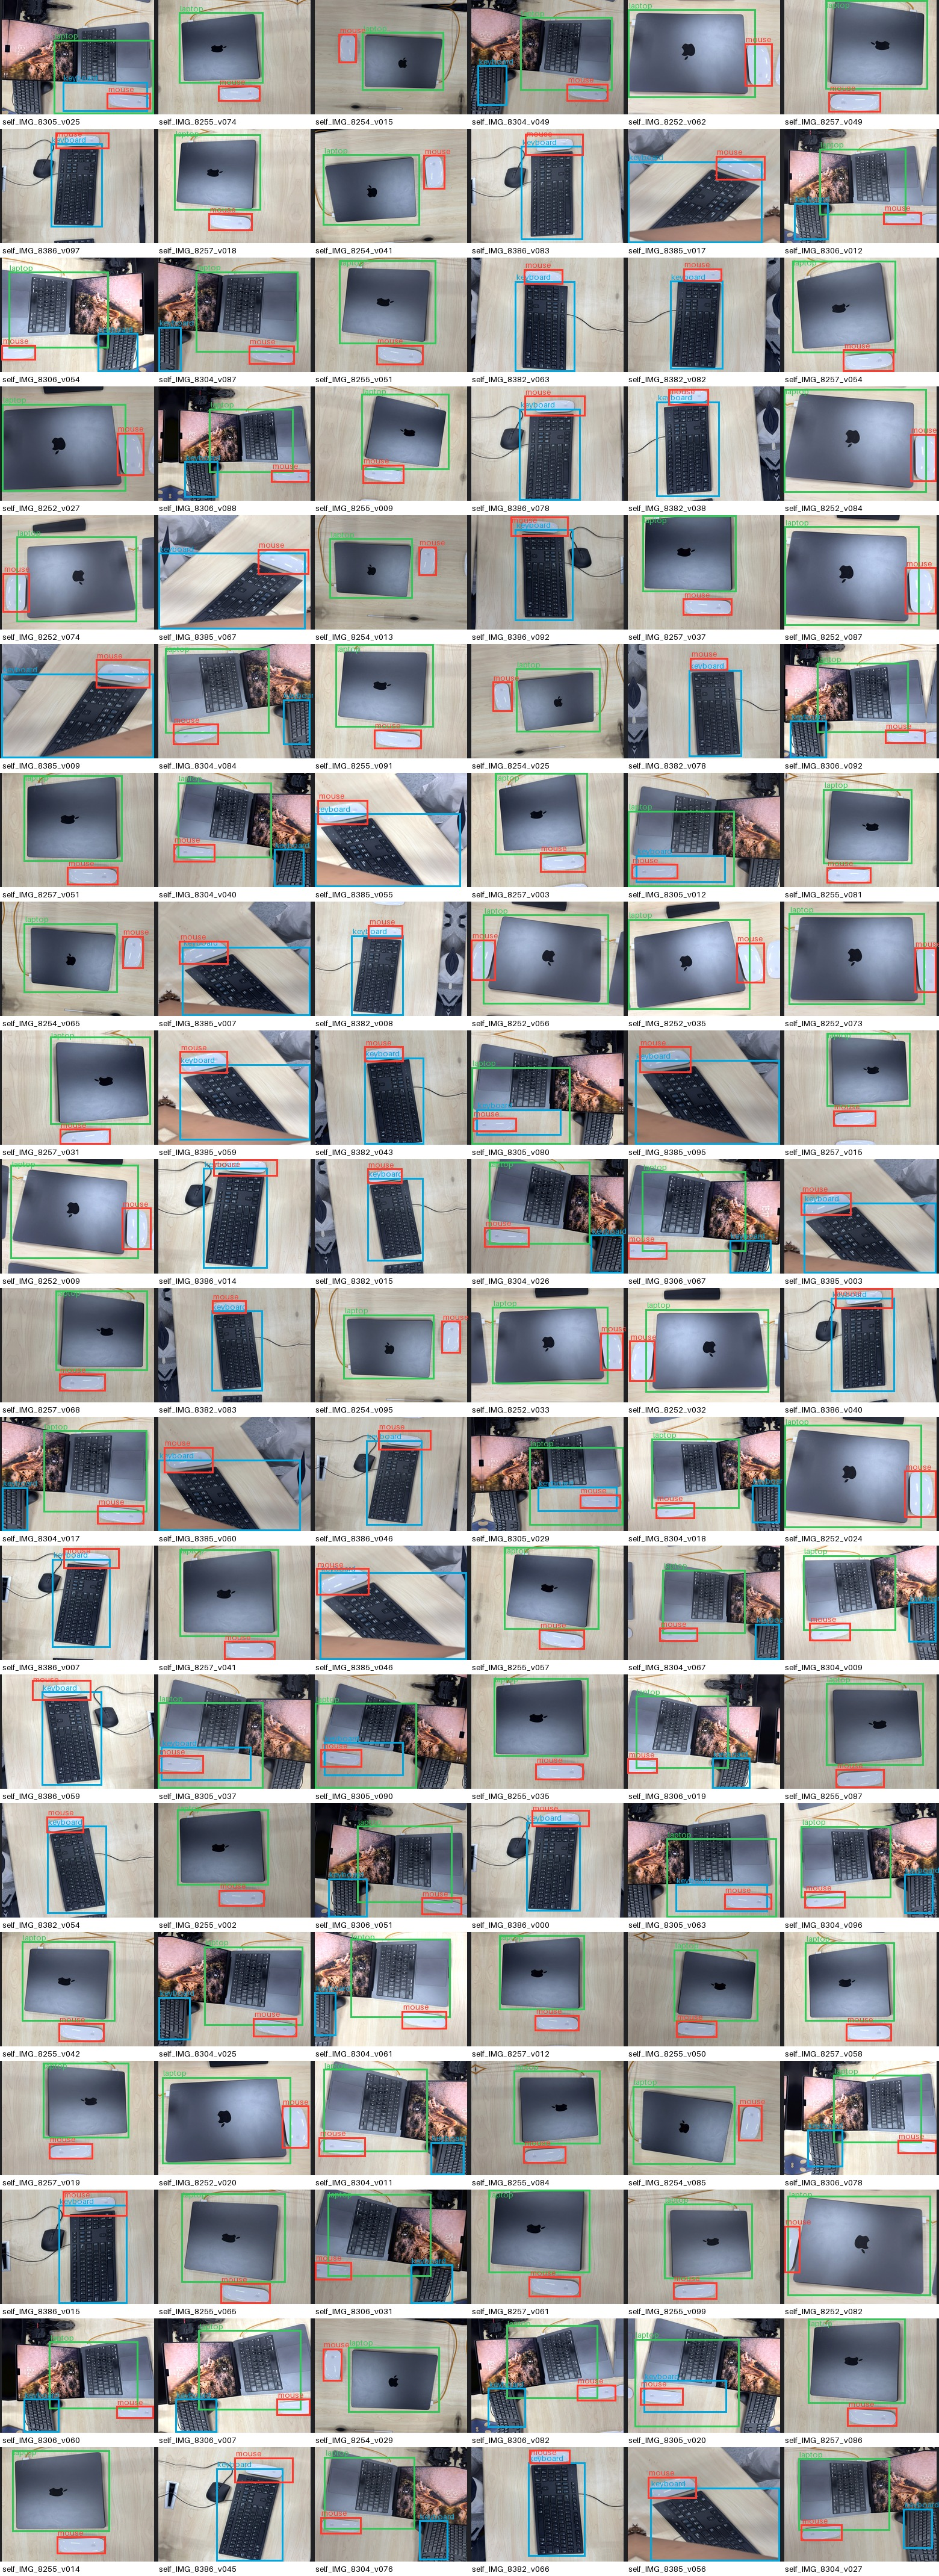
\includegraphics[trim=0 2140 0 0,clip,width=0.485\textwidth]{self_derived_contact_sheet.jpg}\hfill
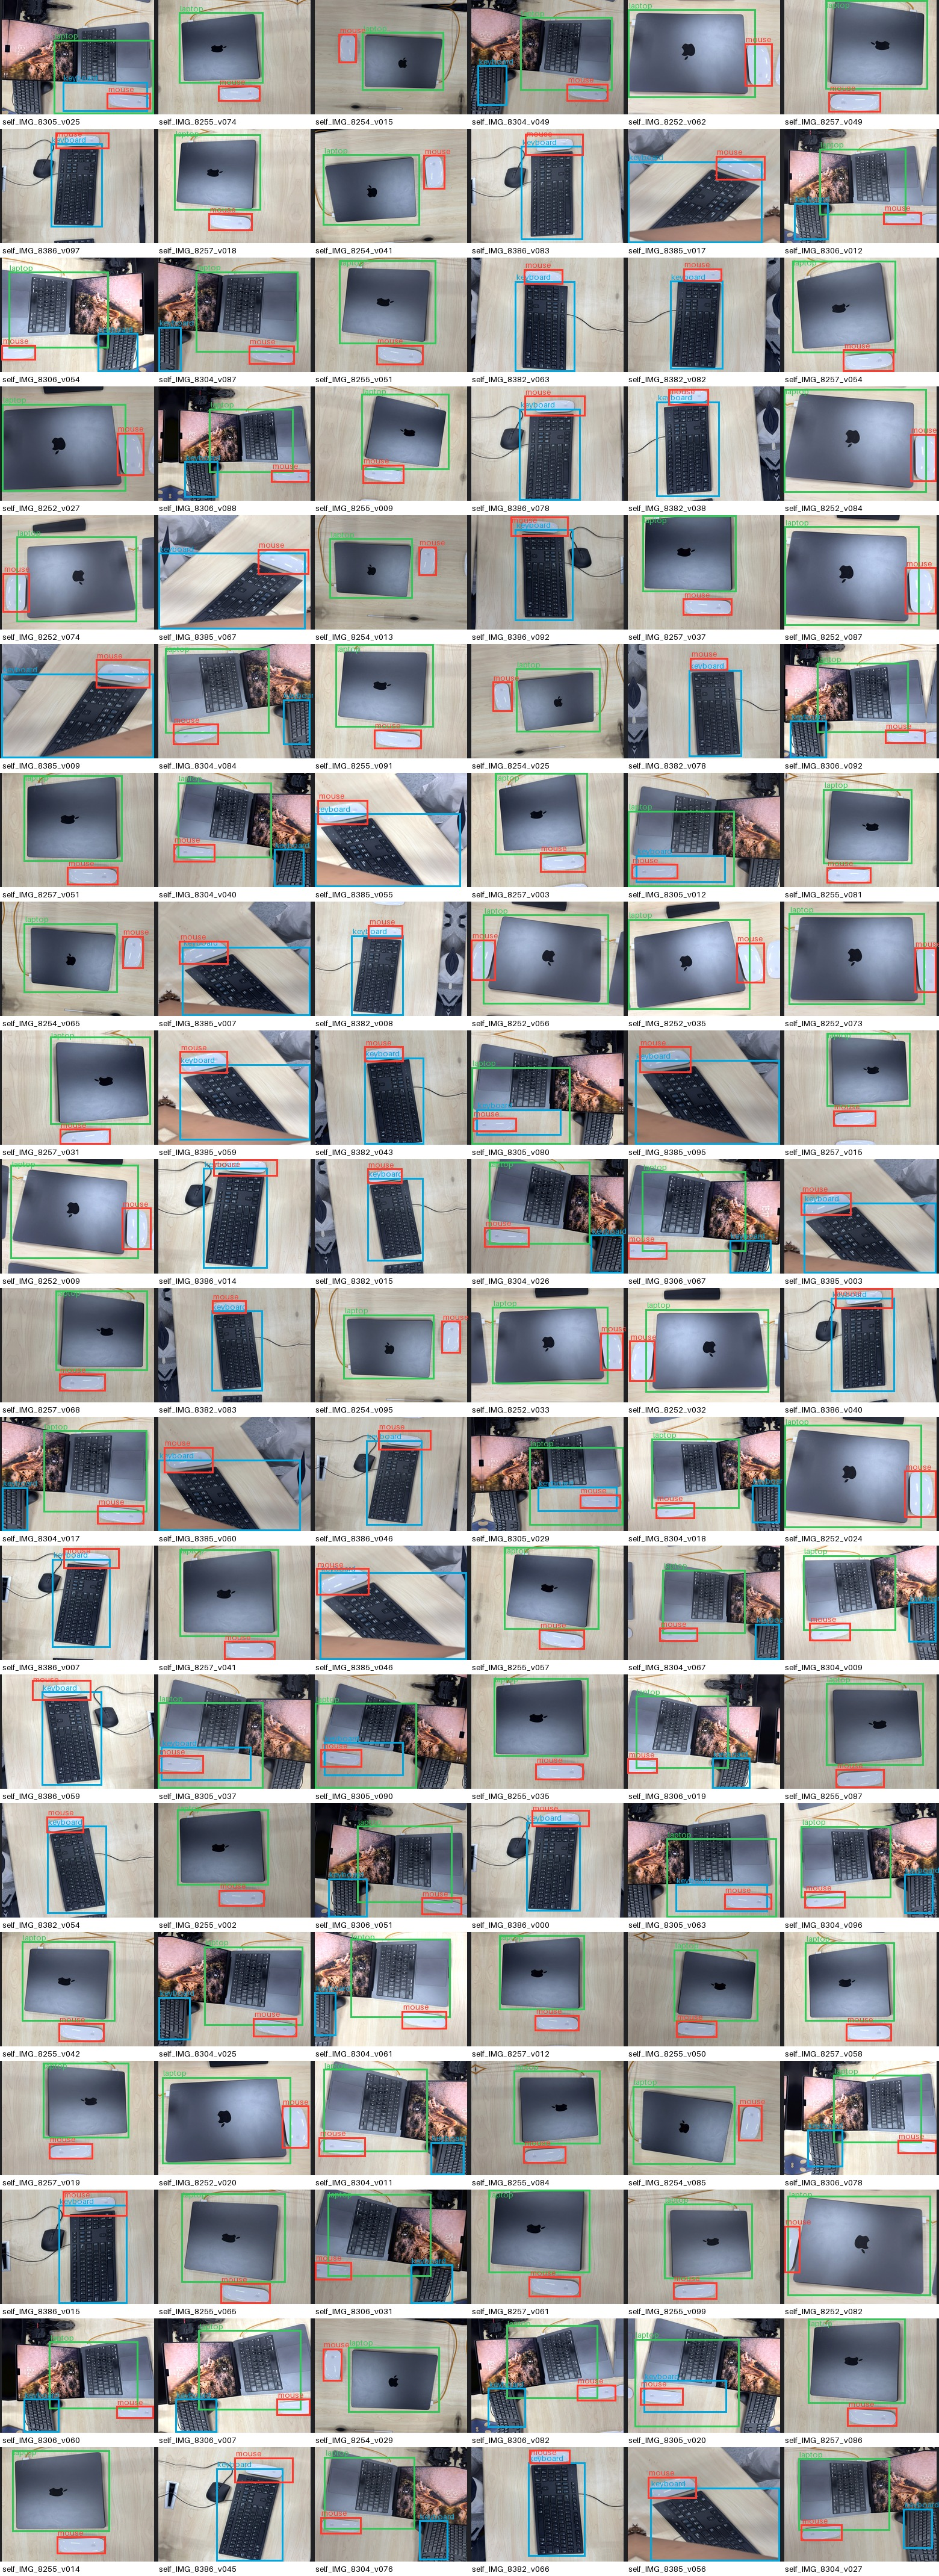
\includegraphics[trim=0 0 0 2140,clip,width=0.485\textwidth]{self_derived_contact_sheet.jpg}
\caption{自主采集来源素材的增强与标注样例。}
\label{fig:selfsamples}
\end{figure*}

五类目标框数量如表\ref{tab:classdist}所示。laptop 数量最多，占全部框的29.96\%；headphones 数量最少，占10.24\%。类别分布并非严格均衡，因此总体指标之外还需检查逐类 Precision、Recall 和 AP，避免样本较多的类别掩盖弱类别表现。

\begin{table}[t]
\caption{五类目标框分布}
\label{tab:classdist}
\centering
\footnotesize
\begin{tabular}{lrr}
\toprule
类别 & 目标框数 & 比例（\%） \\
\midrule
mouse & 1724 & 20.27 \\
keyboard & 1966 & 23.11 \\
laptop & 2549 & 29.96 \\
cup & 1397 & 16.42 \\
headphones & 871 & 10.24 \\
\midrule
合计 & 8507 & 100.00 \\
\bottomrule
\end{tabular}
\end{table}

\section{实验设置与评价方法}

\subsection{实验环境}

模型训练与软件测试在 macOS 平台完成，处理器为 Apple M4，Python 版本为3.12.4，PyTorch 版本为2.13.0，Ultralytics 版本为8.4.133，计算设备使用 MPS。训练输入尺寸与测试输入尺寸均设为640。最佳模型来自第12轮，其验证集 Precision 为0.7407、Recall 为0.7512、\mAPfifty{} 为0.7334、\mAPcoco{} 为0.4621。

\subsection{评价指标与测试协议}

设真正例、假正例和假负例分别为 $TP$、$FP$ 和 $FN$，则 Precision 与 Recall 定义为
\begin{equation}
P=\frac{TP}{TP+FP},\qquad R=\frac{TP}{TP+FN}.
\end{equation}
预测框与真实框的交并比为
\begin{equation}
\mathrm{IoU}=\frac{|B_p\cap B_g|}{|B_p\cup B_g|},
\end{equation}
其中 $B_p$ 和 $B_g$ 分别为预测框与真实框。\mAPfifty{} 在 IoU 阈值0.5下计算各类别 AP 的均值，\mAPcoco{} 则在0.5至0.95、步长0.05的多个阈值上平均，因而对边界框定位更严格\cite{lin2014coco,ultralyticsval}。

实验设置三种互补测试。第一种在650张测试图像上计算总体及逐类检测指标，并生成 PR 曲线与混淆矩阵。第二种从已保存的单目标图片中按每类4张组成20样本集合，以指定类别是否被检出作为正确判据，直接计算课程协议下的正确率。第三种在固定视频上先预热20帧，再统计130帧的端到端处理时间；每帧 FPS 由读取、预处理、推理、后处理和绘制的总耗时换算，保证测试包含完整软件链路。

\section{实验结果与分析}

\subsection{测试集总体结果}

表\ref{tab:metrics}列出了650张测试图像上的结果。模型总体 Precision 为0.8385，说明保留检测中误检比例较低；Recall 为0.7697，表明漏检仍是主要误差来源。总体 \mAPfifty{} 达到0.8386，而更严格的 \mAPcoco{} 为0.5735。两个 mAP 指标之间相差0.2651，说明模型在判断目标存在与类别方面表现较好，但在较高 IoU 阈值下的边界定位仍有提升空间。

\begin{table}[t]
\caption{测试集总体与逐类检测指标}
\label{tab:metrics}
\centering
\scriptsize
\begin{tabular}{lrrrr}
\toprule
类别 & Precision & Recall & \mAPfifty{} & \mAPcoco{} \\
\midrule
mouse & 0.9325 & 0.9101 & 0.9501 & 0.7546 \\
keyboard & 0.8346 & 0.8469 & 0.9012 & 0.6361 \\
laptop & 0.9121 & 0.7529 & 0.8640 & 0.4599 \\
cup & 0.9091 & 0.7409 & 0.8571 & 0.6751 \\
headphones & 0.6041 & 0.5978 & 0.6203 & 0.3419 \\
\midrule
总体 & 0.8385 & 0.7697 & 0.8386 & 0.5735 \\
\bottomrule
\end{tabular}
\end{table}

mouse 的四项指标最高或接近最高，其中 \mAPfifty{} 为0.9501、Recall 为0.9101，显示其外观与标注边界较易被当前模型学习。keyboard 的 \mAPfifty{} 为0.9012，在打开笔记本产生嵌套框的情况下仍保持较高召回。laptop 的 Precision 达到0.9121，但 Recall 为0.7529，且 \mAPcoco{} 降至0.4599，反映整机框在遮挡、开合姿态或边缘截断时更容易出现定位偏差。

逐类结果中，耳机的表现相对较弱，其 Precision、Recall 和 \mAPfifty{} 分别为0.6041、0.5978和0.6203。该类别目标框数量最少，且耳罩、头梁、折叠姿态和遮挡形式变化较大。数据数量与表现之间只能视为相关线索，不能单独证明因果关系；但该结果明确指出，后续数据迭代应优先增加不同姿态、尺度和背景下的耳机样本。归一化混淆矩阵见图\ref{fig:confusion}，可用于观察弱类别的漏检和类别混淆。

\begin{figure}[t]
\centering
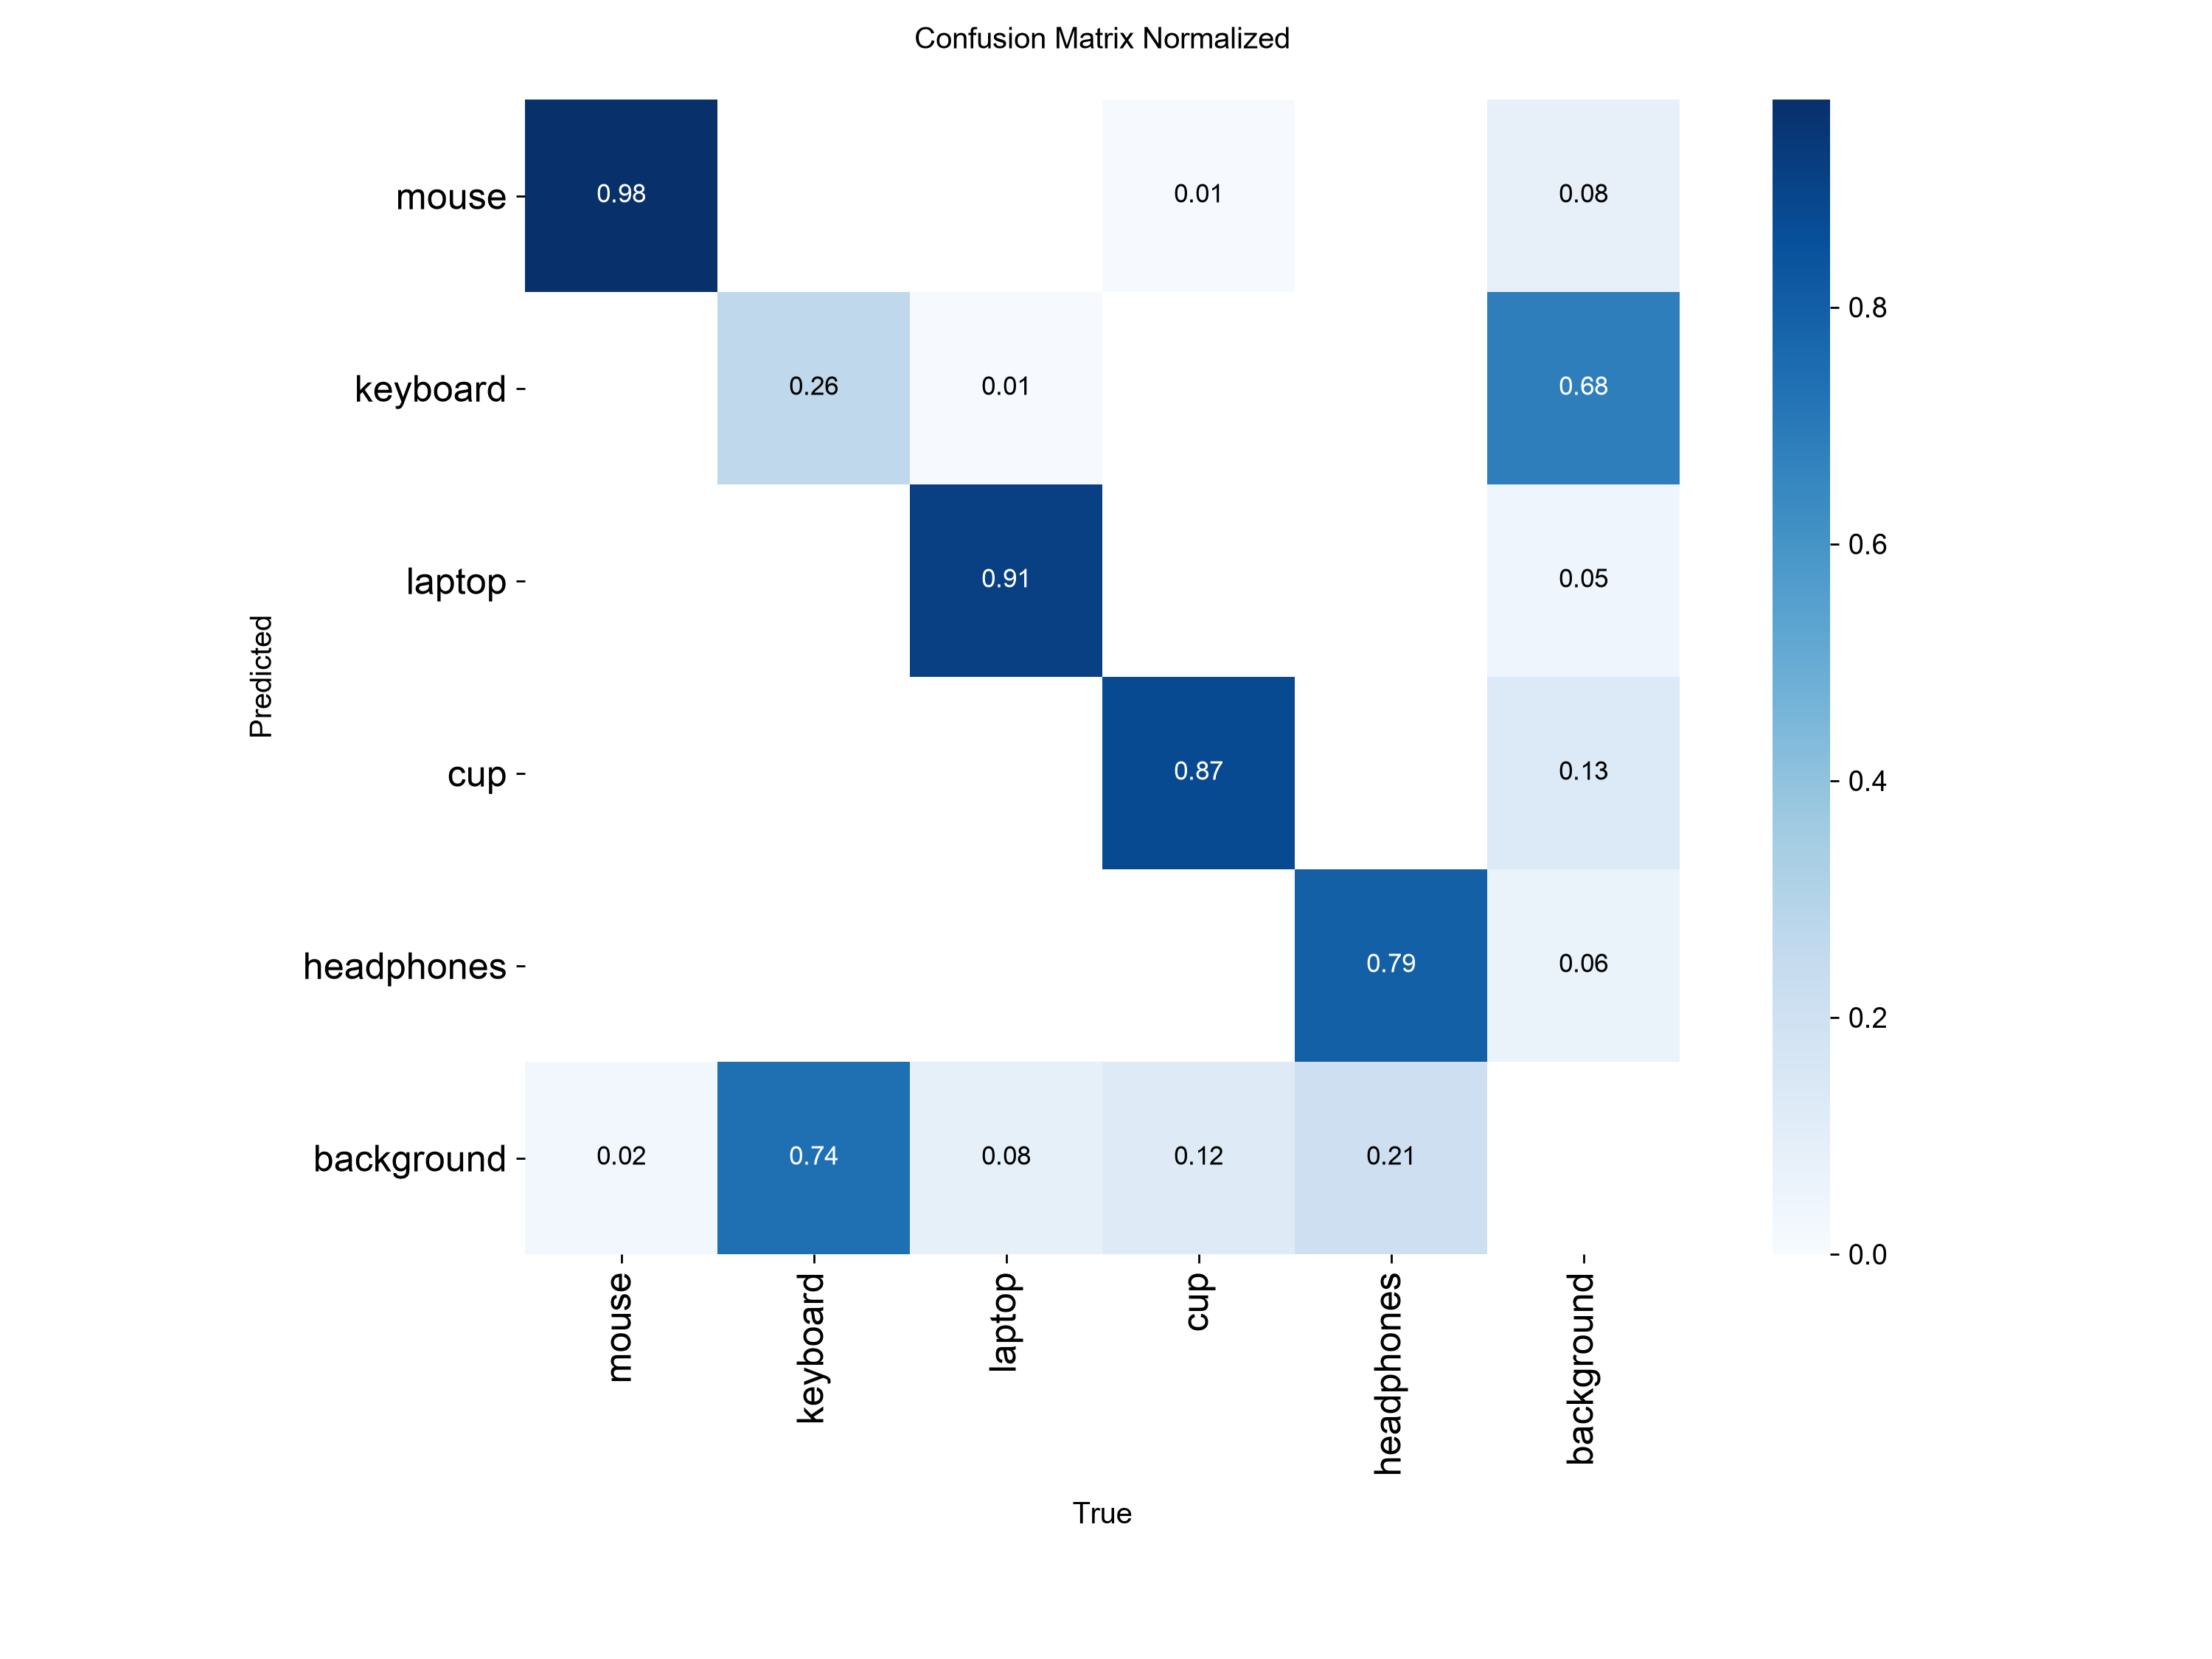
\includegraphics[width=0.92\columnwidth]{confusion_matrix_normalized.png}
\caption{650张测试图像上的归一化混淆矩阵。}
\label{fig:confusion}
\end{figure}

\subsection{训练过程与20样本测试}

图\ref{fig:training}给出了12轮训练的损失与验证指标变化。训练后期验证集 mAP 保持上升，第12轮获得本次最佳权重。由于训练从已有五类模型继续微调，较短训练周期即可进入稳定区间。曲线未出现验证指标持续恶化的明显阶段，最佳权重与最后一轮权重在本次训练中来自同一轮次。

\begin{figure*}[t]
\centering
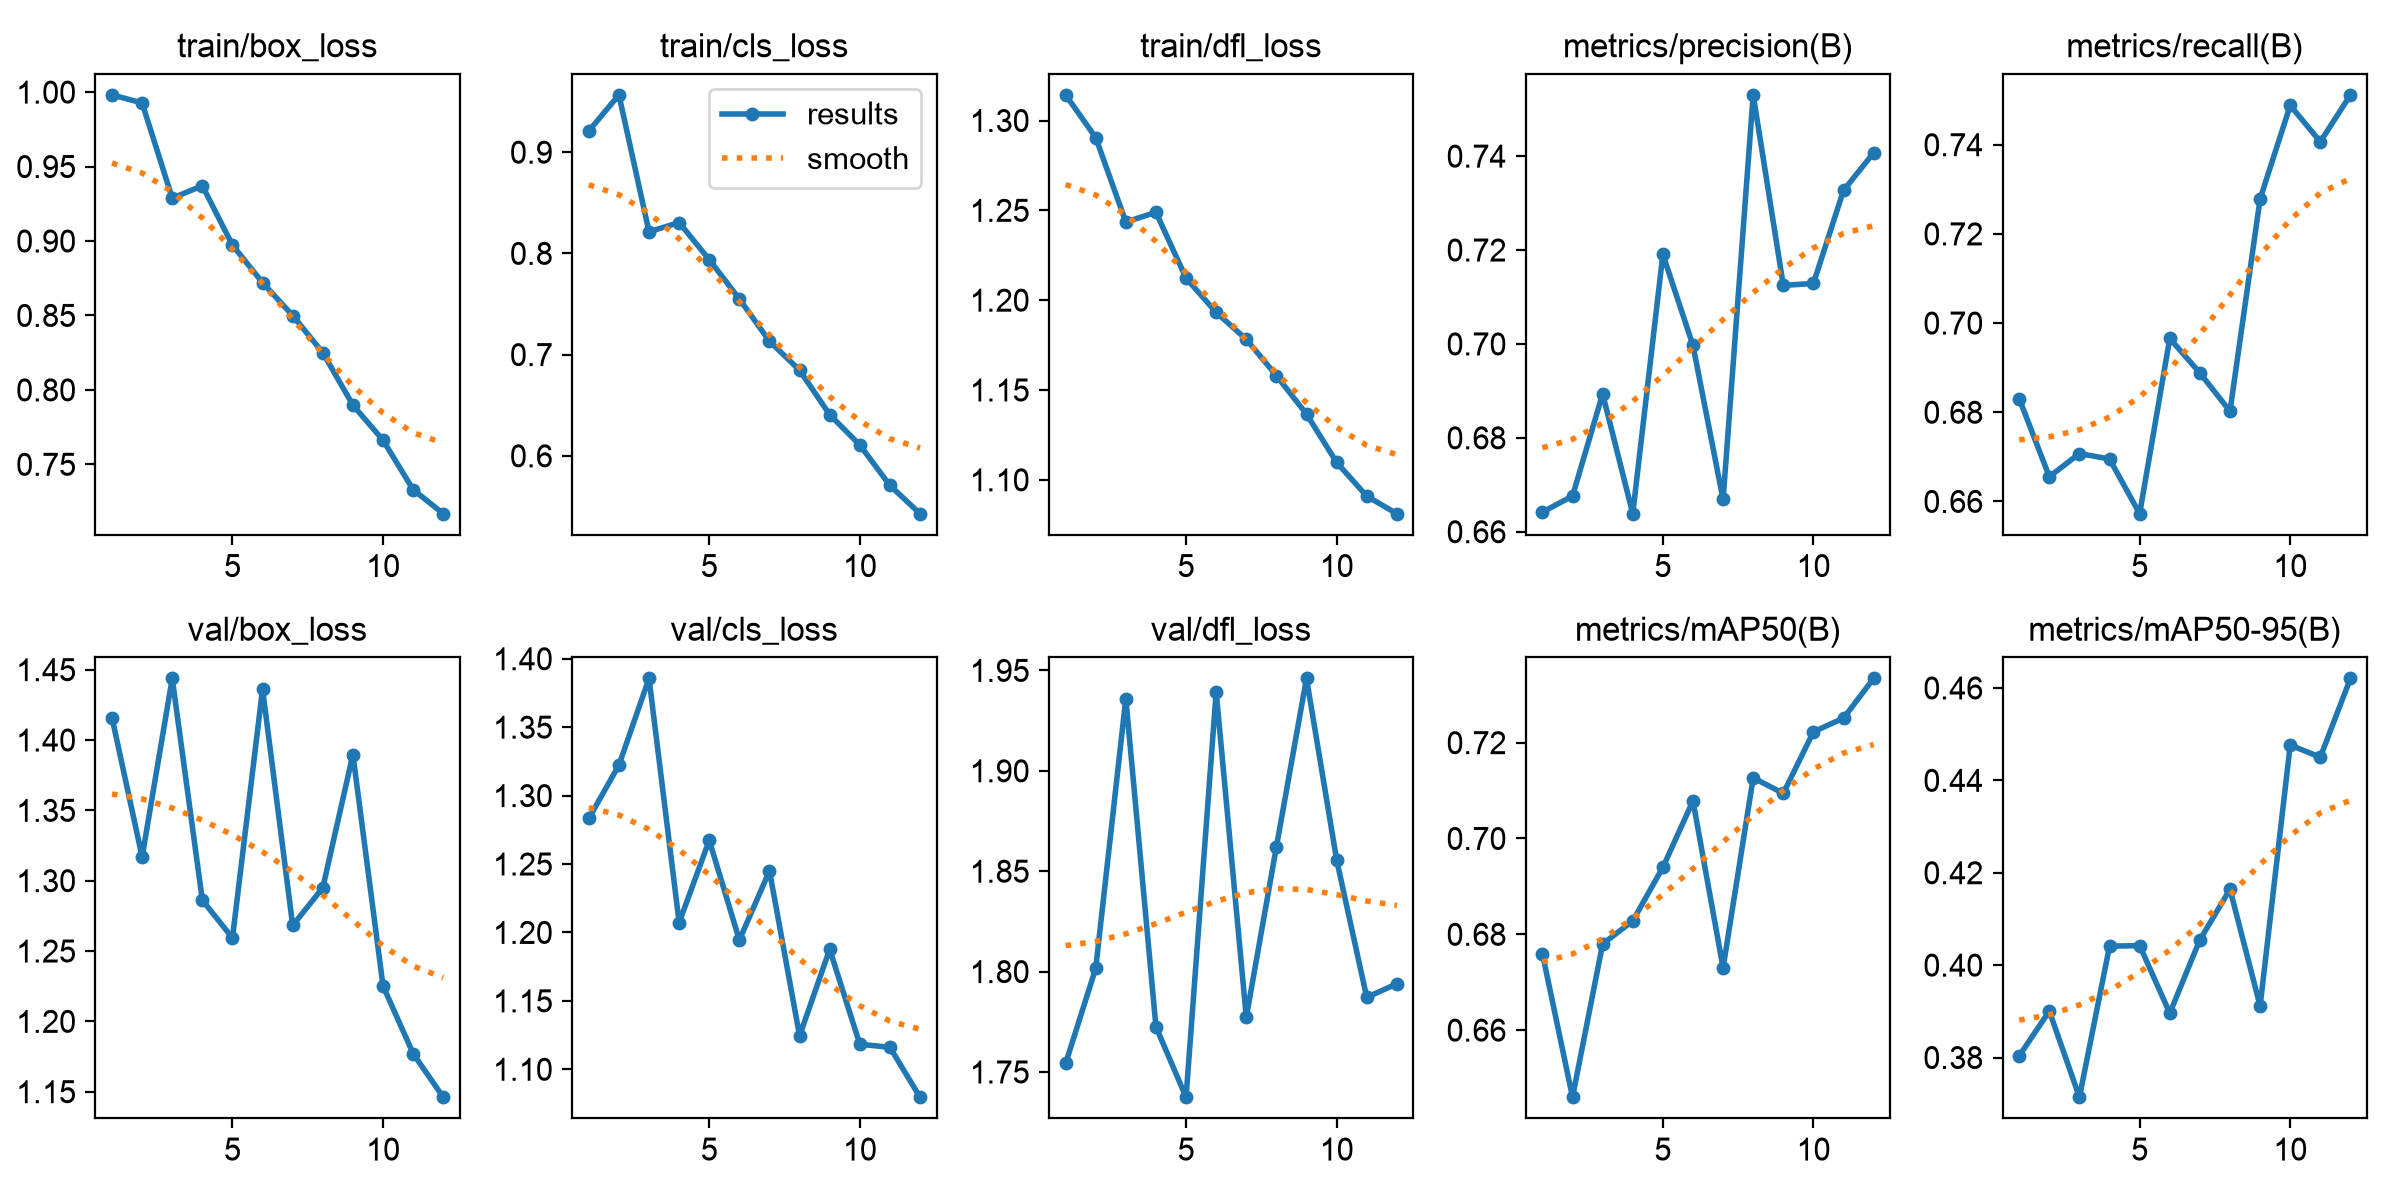
\includegraphics[width=0.88\textwidth]{results.png}
\caption{YOLO11n 在12轮迁移学习中的损失和验证指标曲线。}
\label{fig:training}
\end{figure*}

20样本测试中，模型正确检出19张，正确率为95\%，高于实验要求的80\%。唯一错误为 laptop 漏检，模型在该图上没有产生达到阈值的 laptop 框。该错误与测试集上 laptop Recall 低于其 Precision 的现象一致：模型一旦输出 laptop 通常具有较高正确性，但部分姿态下会完全漏掉目标。保存错误原图而非只记录汇总数字，使后续复查能够定位到具体背景、尺度和遮挡条件。

\subsection{连续视频性能}

固定视频 benchmark 共统计130个计时帧。平均模型推理耗时为10.087 ms，平均端到端耗时为16.554 ms，对应平均60.409 FPS；最低瞬时速度为34.733 FPS，最大模型推理耗时为13.450 ms。模型推理只占端到端时间的一部分，其余开销来自视频读取、图像预处理、检测框绘制和结果组织。即使纳入这些环节，连续处理速度仍显著高于实验规定的5 FPS 阈值。表\ref{tab:summary}汇总了主要实验结果。

\begin{table}[t]
\caption{主要实验结果汇总}
\label{tab:summary}
\centering
\footnotesize
\begin{tabular}{p{0.48\columnwidth}p{0.39\columnwidth}}
\toprule
测试项目 & 结果 \\
\midrule
测试集规模 & 650张，1107个目标框 \\
总体 \mAPfifty{} / \mAPcoco{} & 0.8386 / 0.5735 \\
20样本正确率 & 19/20，95\% \\
平均推理耗时 & 10.087 ms \\
平均端到端速度 & 60.409 FPS \\
最低瞬时速度 & 34.733 FPS \\
\bottomrule
\end{tabular}
\end{table}

\section{ROS2 通信与边缘部署设计}

\subsection{检测节点与主题接口}

ROS2 检测节点将模型推理封装为独立进程，支持 USB 摄像头和图像主题两种输入方式。摄像头模式由节点直接读取视频帧，图像主题模式订阅 \texttt{/camera/image\_raw}，便于与已有相机驱动组合。节点加载统一模型配置，对每帧执行推理，并把结果发布到两个输出主题。\texttt{/object\_detection/result} 使用字符串承载 JSON，字段包括时间戳、帧号、FPS、类别编号、类别名称、置信度和边界框；\texttt{/object\_detection/image} 发布绘制检测框后的 \texttt{sensor\_msgs/Image}。

这一双主题设计兼顾机器可读结果与人工可视化。控制或记录节点只需订阅 JSON 结果，不必传输完整图像；调试界面则可直接显示带框图像。ROS2 的发布/订阅机制允许多个订阅者共享同一数据流\cite{ros2topics}。在课程演示中，可使用 \texttt{ros2 topic echo} 检查字段内容，以 \texttt{ros2 topic hz} 统计消息接收频率，并通过 \texttt{rqt\_image\_view} 显示检测图像。

\subsection{边缘推理流程}

边缘部署以训练得到的 \texttt{best.pt} 为起点。PyTorch 权重可直接用于功能验证，也可以通过 ONNX 作为中间表示导入 TensorRT。TensorRT 在构建阶段根据目标 GPU 为各层选择实现并生成序列化 engine，运行阶段加载 engine 完成推理\cite{nvidiatensorrt}。由于序列化 engine 默认与操作系统、CPU 架构、GPU 型号和 TensorRT 版本相关，工程流程在目标设备上完成 engine 构建，并固定输入尺寸与精度模式。

部署程序沿用训练时的五类顺序和640像素输入，采用 FP16 时保持相同的置信度与 NMS 参数。性能测试先执行预热帧以降低首次加载和内核初始化的影响，再统计固定帧数的端到端 FPS。若资源受限，可依次比较640、512和416输入尺寸，但每次调整后均需重新执行20样本测试，以保证速度优化没有破坏规定的检测正确率。由此，模型、摄像头、结果保存与 ROS2 通信形成统一的边缘视觉执行链路。

\IEEEtriggeratref{6}
\bibliographystyle{IEEEtran}
\bibliography{references}

\end{document}
